\chapter{Marco de Referencia}

Desde finales del siglo pasado, los avances tecnológicos en la miniaturización de la electrónica y los componentes mecánicos han allanado el camino para la creación y desarrollo de objetos voladores de pequeñas dimensiones, tales como aviones y helicópteros, los cuales están adquiriendo cada vez más habilidades para realizar vuelos de forma autónoma. Estos dispositivos son popularmente conocidos como drones, un término derivado del inglés \say{abejorros}, y se consideran máquinas voladoras autónomas o semi-autónomas capaces de llevar a cabo misiones de vuelo. En el ámbito internacional, se les conoce como UAVs del inglés \say{Unmanned Aerial Vehicles}, y representan una tecnología compleja cuyo control presenta desafíos, dado que sus características aerodinámicas son similares a las de las aeronaves convencionales~\cite{eisenbeiss2004mini}.

El estudio de estos dispositivos despierta un gran interés debido a su versatilidad y capacidad de maniobra, lo que les permite llevar a cabo una amplia gama de tareas en diversas aplicaciones, tales como el uso civil, militar y aeroespacial~\cite{nawaz2019applications, shakhatreh2019unmanned, xiaoning2020analysis}. En la figura~\ref{fig1_aplicacion_UAV}, se presenta una clasificación detallada de las aplicaciones más importantes de los UAVs.

\begin{figure}[H]
    \centering
    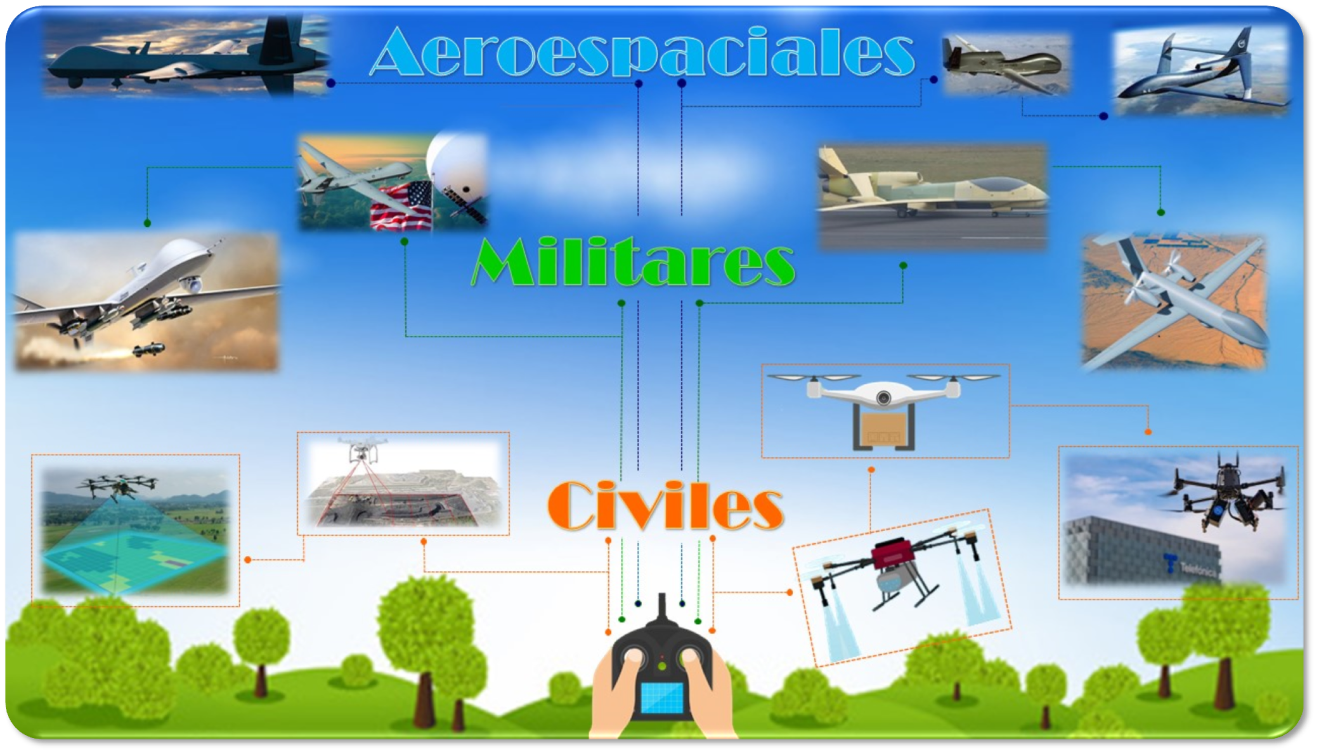
\includegraphics[width=16cm, height=7.5cm]{imagenes/Aplicaciones_UAV.png}
    \caption{Áreas de aplicación UAVS.}
    \label{fig1_aplicacion_UAV}
\end{figure}

\section{Antecedentes.}

Los drones han atraído la atención de la comunidad investigadora que trabaja tanto en el campo militar como en el civil, con una gran cantidad de usos que han sido propuestos por los grupos de investigación, debido a sus características como capacidad y configuraciones, donde el helicóptero de cuatro rotores tiene el mayor número de citas en la literatura de control y ha sido ampliamente investigado para pruebas tanto en interiores como en exteriores.

\section{Objetivo General}

Desarrollar un sistema web para el control y administracion de un taller de reparaciones de equipos de TI, mediante el uso de framework de Laravel para el seguimiento de ordenes de trabajo, la gestion de inventario y la comunicacion con los clientes.

\section{Objetivos Especificos}
\begin{enumerate}
\item Analizar los requerimientos operativos y el flujo de trabajo del taller mediante entrevistas e instrumentos de recoleccion de datos para los modulos clave del sistema.
\item Diseñar la arquitectura de software y el modulo base de datos, utilizando el lenguaje modelado para la estructura y escalabilidad de la información.
\item Implementar el modulo de trazabilidad de un panel de control interactivo para el seguimiento del estado de cada reparacion en tiempo real.
\end{enumerate}

\section{Alcance}

El presente proyecto abarca el análisis, diseño e implementación de un sistema web desarrollado con el framework Laravel para la gestión centralizada de un taller de reparación de equipos de Tecnologías de la Información (computadoras, impresoras y periféricos). El sistema contempla los siguientes módulos y funcionalidades principales:

\begin{itemize}
    \item \textbf{Gestión de usuarios y control de acceso por roles:} Administración de cuentas de usuario, inicio y cierre de sesión, recuperación de contraseña mediante token por correo electrónico y asignación de permisos específicos para cinco roles: Administrador, Recepción, Técnico, Almacén y Cliente.
    \item \textbf{Gestión de clientes y recepción de equipos:} Registro y actualización de datos de clientes, control de antigüedad e historial de servicio, así como el ingreso de dispositivos con folio único, registro de características físicas, número de serie, accesorios y evidencias fotográficas.
    \item \textbf{Diagnóstico técnico y gestión de cotizaciones:} Captura de fallas detectadas, pruebas técnicas y posibles soluciones; generación de cotizaciones con control de versiones, mano de obra, refacciones, vigencia y aplicación de descuentos autorizados.
    \item \textbf{Flujo de aprobaciones y seguimiento de reparaciones:} Registro de aceptación o rechazo de presupuestos por parte del cliente o administrador, asignación de técnicos, bitácora de tareas, tiempos de trabajo, registro de incidencias y actualización de estados en tiempo real.
    \item \textbf{Control de almacén e inventario:} Administración de entradas, salidas, existencias mínimas y reserva de refacciones vinculadas a órdenes autorizadas, así como alertas por faltantes de material o reemplazo de herramientas.
    \item \textbf{Gestión de pagos, entregas y garantías:} Registro de anticipos (50\,\% requerido para iniciar la reparación, salvo excepción autorizada), pagos parciales, liquidaciones, emisión de comprobantes de pago, validación de pruebas finales previas a la entrega y administración de garantías y reingresos.
    \item \textbf{Portal de consulta para clientes, reportes y bitácora:} Interfaz para que el cliente consulte el avance de sus órdenes, apruebe o rechace cotizaciones y verifique sus pagos y garantías, complementada con un módulo de reportes operativos y auditoría de acciones relevantes en el sistema.
\end{itemize}

\section{Limitación}

Durante el desarrollo y operación del sistema se consideran las siguientes limitaciones técnicas y operativas:

\begin{itemize}
    \item \textbf{Procesamiento de pagos en línea:} El sistema registra y controla anticipos, pagos parciales, saldos pendientes y comprobantes, pero no integra pasarelas de pago bancarias en línea ni terminales punto de venta físicas; la validación del cobro se realiza mediante registro administrativo.
    \item \textbf{Facturación electrónica fiscal:} Los comprobantes generados por el sistema son de carácter interno y de control operativo para el taller y el cliente, por lo que no sustituyen comprobantes fiscales digitales (CFDI) ante autoridades tributarias.
    \item \textbf{Adquisición y compras automatizadas a proveedores:} El módulo de almacén notifica faltantes de inventario y necesidades de reposición de herramientas al administrador, pero no realiza órdenes de compra automáticas ni se conecta con sistemas externos de proveedores.
    \item \textbf{Dependencia de conectividad e infraestructura:} Al ser una aplicación web accesible desde navegadores modernos, su disponibilidad durante el horario operativo del taller depende de la conexión a red y de la infraestructura del servidor donde se aloje.
    \item \textbf{Alcance del diagnóstico por software:} El sistema documenta y da trazabilidad a los diagnósticos, pruebas y tiempos de reparación capturados por el personal técnico, pero no ejecuta diagnósticos de hardware o telemetría de forma automatizada sobre los equipos recibidos.
    \item \textbf{Restricciones de flujo operativo:} Conforme a las reglas de negocio establecidas, el sistema no permite iniciar reparaciones sin cotización vigente aprobada y anticipo registrado (salvo autorización expresa del administrador), ni permite cancelar órdenes por vía ordinaria una vez iniciada la reparación.
\end{itemize}

\section{Problemática}


\section{Justificación}

